% !TEX program = xelatex
% !BIB program = bibtex

\documentclass[UTF8,cs4size]{ctexart}

% layout
\usepackage[left=3cm,right=3cm]{geometry}
\usepackage{paralist}
\linespread{1.25}
% \ctexset{
%   section = {
%     name = \S
%   },
%   subsection/name = \S,
%   subsubsection/name = \S
% }
% \makeatletter
% \def\@seccntformat#1{%
%   \expandafter\ifx\csname c@#1\endcsname\c@section
%   Section \thesection:
%   \else
%   \csname the#1\endcsname\quad
%   \fi}
% \makeatother
 
% page headings
\usepackage{fancyhdr}
\setlength{\headheight}{15.2pt}
\pagestyle{fancy}
\lhead{}
\rhead{M201873026 刘一龙}
\cfoot{\thepage}
% \makeatletter
% \let\headauthor\@author
% \makeatother

% footnote
\renewcommand\thefootnote{\fnsymbol{footnote}}

% url/ref
\usepackage{hyperref}
\hypersetup{
  colorlinks,
  citecolor=black,
  filecolor=black,
  linkcolor=black,
  urlcolor=black,
  pdfauthor={刘一龙},
  pdftitle={面向对象方法学实战 1}
}

% vertical centering title page
\usepackage{titling}
% \renewcommand\maketitlehooka{\null\mbox{}\vfill}
\renewcommand\maketitlehookd{\vfill\null}

% table of contents
\usepackage{tocloft}
\renewcommand\cftsecfont{\normalfont}
\renewcommand\cftsecpagefont{\normalfont}
\renewcommand{\cftsecleader}{\cftdotfill{\cftsecdotsep}}
\renewcommand\cftsecdotsep{\cftdot}
\renewcommand\cftsubsecdotsep{\cftdot}
\renewcommand\cftsubsubsecdotsep{\cftdot}
\renewcommand{\contentsname}{\hfill\bfseries\Large 目录\hfill}   
\setlength{\cftbeforesecskip}{10pt}

% figures
\usepackage{graphicx}
\graphicspath{figures/}
% \newcommand\figureht{\dimexpr
%   \textheight-3\baselineskip-\parskip-.2em-
%   \abovecaptionskip-\belowcaptionskip\relax}

% tables
\usepackage{caption} 
\captionsetup[table]{skip=10pt}

% math, algorithms, code
\usepackage{amsmath,amssymb,url}
\usepackage{algorithm,algorithmicx,algpseudocode}
\usepackage{listings}

\lstset{
   extendedchars=true,
   basicstyle=\footnotesize\ttfamily,
   showstringspaces=false,
   showspaces=false,
   numbers=left,
   numberstyle=\footnotesize,
   numbersep=9pt,
   tabsize=2,
   breaklines=true,
   showtabs=false,
   captionpos=b
}

% bibliography
\usepackage[super,square,comma,sort]{natbib} % for \citet and \citep
\renewcommand{\refname}{参考文献}
% \begin{filecontents}{report.bib}
% \end{filecontents} 

% appendix
\usepackage{appendix}

\title{{\LARGE \textbf{面向对象方法学实战 1}}\\  \vspace{7cm}}
\author{计算机科学与技术学院\\ 硕1801班\\ \textbf{M201873026}\\ \textbf{刘一龙}}
\date{2018年11月}

\begin{document}

\pagenumbering{gobble} % no page number
\maketitle
\newpage
\tableofcontents
\newpage

\pagenumbering{arabic}

\section{主要需求}
GBA(GoBang Ai)系统\footnote{本系统的在线版已发布于~\href{http://ai.hust.cf}{ai.hust.cf},
可以访问该网站与 GBA 系统进行对弈。},一个基于蒙特卡洛树搜索的简单五子棋人工智能系统,将最简单的基于 UCT 的蒙特卡洛树搜索策略移植到五子棋游戏上。
GBA 系统实现了基本的对弈功能,但受限于浏览器的运算能力,
其棋力还十分地孱弱。在使用随机模拟策略时,其落子选择表现异常糟糕。
利用计分板策略进行优化后,使得其消除了极为糟糕的落子选择(如未能杀 4)。
\clearpage

\section{开发与运行环境}
整个系统用 React~\cite{web:react}框架实现图形界面,并将逻辑模块绑定至相关点击事件。
主游戏流程与人工智能逻辑均由 JavaScript 编写。主要利用到以下工具:

\begin{compactitem}
  \item Git 版本管理工具;
  \item Babel JavaScript 转译器:将 JavaScript 新特性转为 ES5 标准,使其能够运行在低版本的浏览器上;
  \item eslint/stylelint:JavaScript 与 CSS 代码风格检查工具,保证整个工程代码风格一致;
  \item Webpack 构建工具:将 HTML/CSS/JavaScript 文件打包为单一文件,并在这一过程进行代码风格检查、JavaScript 转译、HTML/CSS 混淆 等工作;
  \item NPM 包管理工具:管理工程所需依赖包与工具包。
\end{compactitem}

经过编译、压缩、混淆、打包的 Web 工程通过 Nginx 部署,可以通过~\href{http://ai.hust.cf}{ai.hust.cf}进行访问。

\clearpage

\section{系统结构图}

GBA 系统整体结构如图~\ref{fig:arch}所示。分为两大模块,界面模块与逻辑模块。
界面模块利用组件化开发的思想,将界面分割为多个组件,从而达到代码抽象与复用。
逻辑模块由 Game 模块为入口,通过 AI 与 StateMachine 模块管理游戏策略与游戏流程。

\begin{figure}[htb]
  \centering
  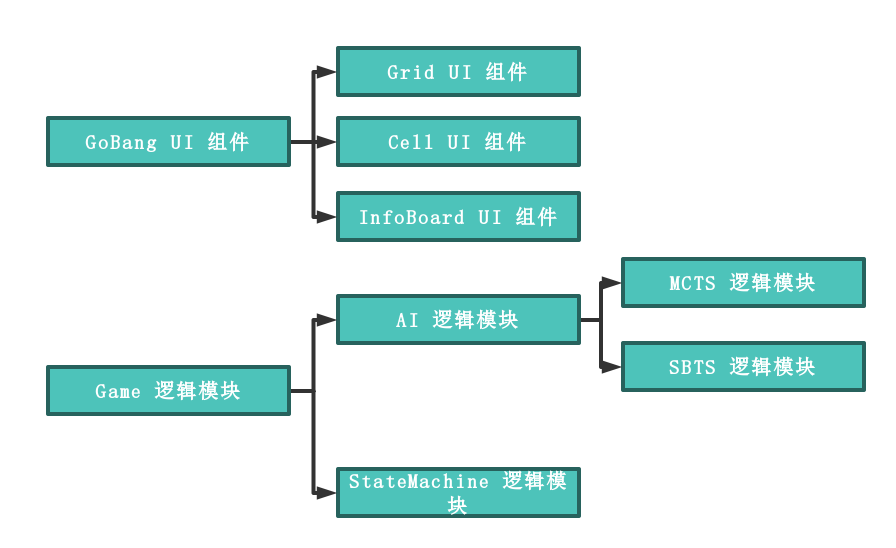
\includegraphics[width=\textwidth,height=7cm]{figures/assign1_arch.png}
  \caption{GBA 系统整体架构图}
  \label{fig:arch}
\end{figure}

\clearpage

\section{界面模块}
本游戏利用 React~\cite{web:react}框架实现,将图形界面封装为三个组件,并将逻辑模块绑定至相关点击事件。
利用 React 框架,遵循组件复用原则,利用 Cell 与 Grid 组件构建了 Gobang,
最后完成了五子棋游戏的图像界面。游戏界面如图~\ref{fig:UI}所示。

\begin{figure}[htb]
  \centering
  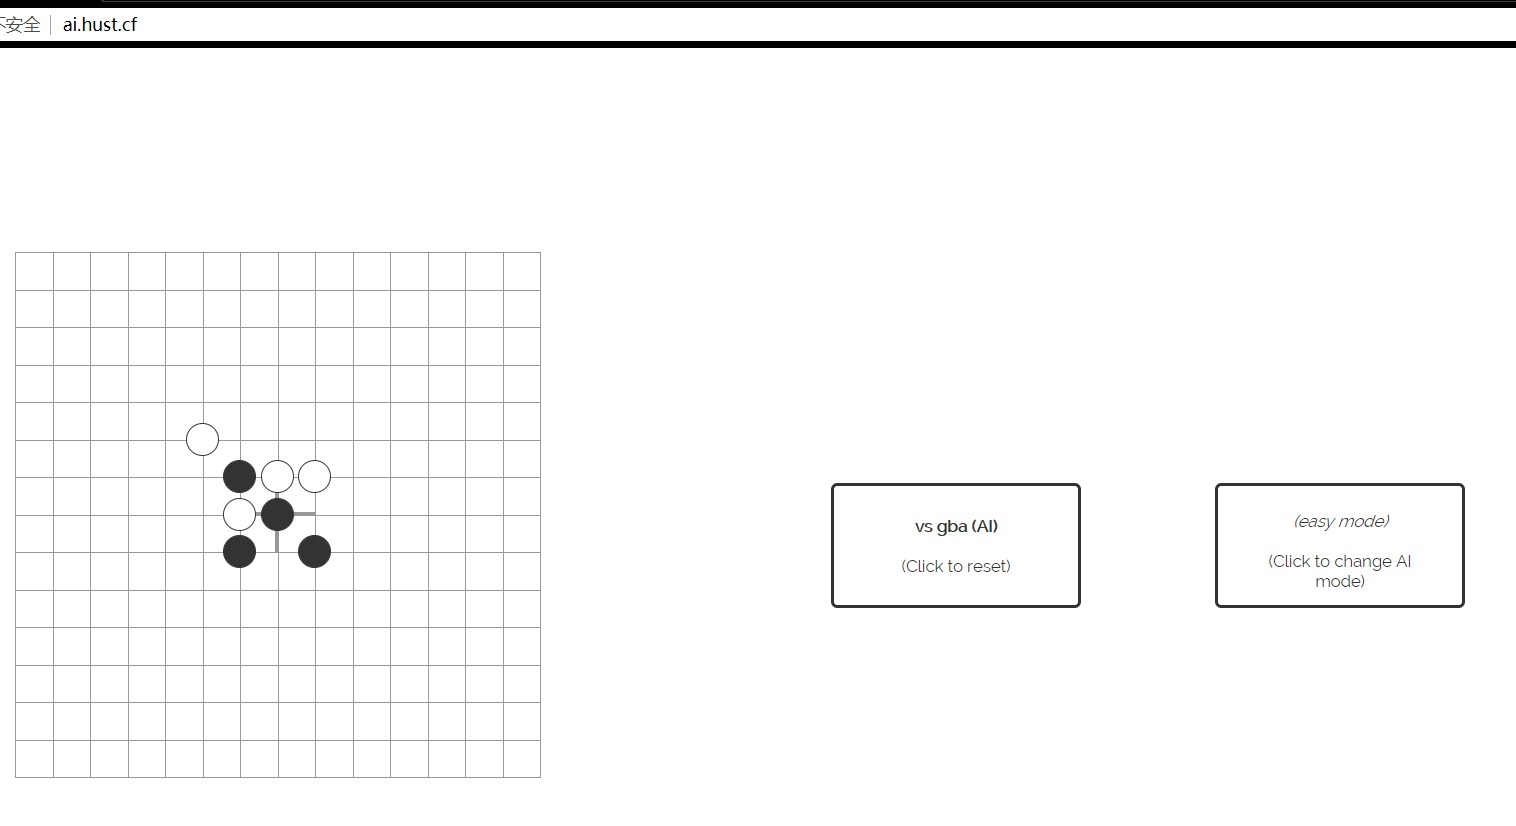
\includegraphics[width=\textwidth,height=7cm]{figures/assign1_UI.png}
  \caption{五子棋游戏主界面}
  \label{fig:UI}
\end{figure}

\clearpage

\section{核心模块}
\subsection{Game 模块}
实现了五子棋游戏的主要逻辑,如 mainLoop、load/storeState、changeGameMode 等。
图形界面的各种点击事件主要是由 Game.js 模块的各个函数进行处理的。
在玩家点击棋盘一个完成落子后,GBA 系统会根据棋局当前局势,利用蒙特卡洛树搜索,在给定的时限内(不同的时限会影响 GBA 系统的强度)给出落子选择。
GBA 系统落子完毕后,玩家可以继续落子,直到决出胜者或达成和局,如流程~\ref{alg:game_main}所示。

\begin{algorithm}
  \floatname{algorithm}{流程}
	\algrenewcommand\algorithmicrequire{\textbf{输入:}}
	\algrenewcommand\algorithmicensure{\textbf{输出:}}
	\caption{游戏主流程}
	\label{alg:game_main}
  \begin{algorithmic}[1]
    \While{未决出胜者 $OR$ 未达成和局}
      \State handleClick($row$, $col$)
      \State $play \gets$ ($row$, $col$)
      \State $newState \gets$ StateMachine.nextState($state$, $play$)
      \State $aiPlay \gets$ AI.bestPlay($newState$)
      \State $newState \gets$ StateMachine.nextState($newState$, $aiPlay$)
    \EndWhile
    \State \textbf{return} $newState$
	\end{algorithmic}  
\end{algorithm}
\clearpage

\subsection{状态管理模块}
StateMachine.js 实现了一些与游戏状态相关的函数,如 nextState、isDeadGame、checkWinner 等。
根据上一次落子后的状态,结合当前轮双方的操作,可以得到下一轮的棋局状态。
这一模块中所有方法都为纯函数,不具有副作用,
从而保证对于给定状态与输入,有着唯一确定的终态。

\subsection{人工智能模块}
AI.js 实现了 GBA 系统中的智能落子功能,利用 SBTC.js 与 MCTS.js 提供的 API 构建完整的五子棋人工智能。
这一对象中使用了策略模式,使得可以在不修改代码的情况下添加/更改智能落子的相关算法。
\clearpage

\section{策略模块}
\subsection{计分板优化策略}
由于性能限制,如果对于所有空格位置处都进行随机搜索的话,
会使得 GBA 系统在限定的时间内(例如 3 秒) 无法得出最有效的落子选择,
使得其最后的落子选择异常糟糕,造成一种“人工智障”的戏剧场面。

利用计分板策略计算当前棋局局势,得出下一步较为优势的落子集合,缩小搜索树,
可以大幅度提升 GBA 系统的落子选择表现。

计分板优化策略根据五子棋的领域知识,对棋盘上所有可行落子的地方进行打分。
如某落子处在某一方向(横/竖/左斜/右斜)形成了“杀4”(即阻断对方五子连续)局势,
则为该处落子增加 50000 分;
如某落子处在某一方向(横/竖/左斜/右斜)形成了“活3”(即本方三子连续,且两端都有空位)局势,
则为该处落子增加 50 分;
如某落子处在某一方向(横/竖/左斜/右斜)形成了“死3”(即本方三子连续,只有一端都有空位)局势,
则为该处落子增加 25 分;
如某落子处在某一方向(横/竖/左斜/右斜)形成了“连5”(即本方五子连续)局势,
则为该处落子增加 90000 分。

采取一系列类似的策略,得到所有可行落子的评分集合,称为计分板。
选取计分板中得分较高的一些落子,放入下一步可行落子集合,
返回给 GBA 系统进行蒙特卡洛树搜索的扩展和模拟阶段。
所有计分策略与对应分数如表~\ref{tab:score_board}所示。

\begin{table}[htbp]
  \caption{计分板策略分数评定}
  \label{tab:score_board}
  \centering
  \begin{tabular}[c]{l|l}
    \hline
    \multicolumn{1}{c|}{\textbf{局势}} & 
    \multicolumn{1}{c}{\textbf{分数}} \\
    \hline
	  杀 2 & 10 \\
	  杀 3(一端空位)& 30 \\
	  杀 3 (两端空位)& 40 \\
	  杀 4(一端空位)& 60 \\
	  杀 4 (两端空位)& 110 \\
	  杀 5 & 50100 \\
	  活 2 & 10 \\
	  死 3 & 25 \\
	  活 3 & 50 \\
	  死 4 & 55 \\
	  活 4 & 100 \\
	  活 5 & 90000 \\
   \hline
  \end{tabular}
\end{table}


\subsection{蒙特卡洛树搜索策略}
MCTS.js 实现了蒙特卡洛树搜索策略,对外提供了 2 个 API:MCTS.runSearch 与 MCTS.bestPlay。

蒙特卡罗树搜索(MCTS),是一种使用随机模拟的最佳优先原则的搜索算法。其基本过程如图~\ref{fig:mcts_phase}所示。
在阶段(1)中,现有信息用于重复选择连续的子节点直到搜索树的末尾。接下来,在阶段(2)中,通过添加节点来扩展搜索树。
然后,在阶段(3)中,模拟运行到最后以确定获胜者。
最后,在阶段(4)中,使用从模拟游戏获得的新信息更新所选路径中的所有节点。
重复运行这种 4 阶段算法,直到收集到足够的信息以产生良好的下一步选择。
重要的是要注意搜索树在结构上与游戏树相同,并且搜索树还包含从模拟中收集的统计信息,搜索树是整个游戏树的一个子集。

\begin{equation}
  \text{UCT} = \frac{w_i}{s_i} + c\sqrt{\frac{\ln{s_p}}{s_i}}
  \label{eq:uct}
\end{equation}

公式~\eqref{eq:uct}称为“UCT 函数”,分为 2 部分:左部为利用值,右部为探索值。其中,
$w_i$ 表示此节点的模拟次数导致获胜;
$s_i$ 表示此节点的模拟总数;
$s_p$ 表示父节点的模拟总数;
$c$ 表示探索参数。
$\frac{w_i}{s_i}$ 表示当前节点的游戏平均胜率,当选择该值较大的节点时,可以很好地利用已知信息做出下一步行动;
$\sqrt{\frac{\ln{s_p}}{s_i}}$ 表示当前节点的模拟频率(被遍历的概率),当选择该值较大的节点(较少模拟)时,可以很好地探索未知路径。
探索参数 $c$ 只是可以选择的一个数字,它控制着等式中利用值与探索值之间的权重大小,选择的通常数字是 $c = \sqrt{2}$。

每次需要在多个子节点之间进行选择时,便使用公式~\eqref{eq:uct}(即 UCT 函数)来获取每个子节点的 UCT 值,并选择具有最大值的子节点。
在选择阶段,使用 UCT 选择功能来决定选择哪个子节点。
反之,UCT 函数使用子节点的获胜次数 $w_i$ 和模拟次数 $s_i$ 以及父节点的模拟次数 $s_p$ 来生成每个子节点的 UCT 值。
此信息在反向传播阶段(即第 4 阶段)更新,因此,获得此迭代的信息将影响下一次迭代的移动选择,依此类推。

重复上述 4 个步骤,进行完足够的迭代后,搜索树上会存储足够的游戏信息,
用于选出下一步理想中最优的行动。
例如,可以简单地选取 $\frac{w_i}{s_i}$ 最大值的子节点作为下一步行动。

\clearpage

\section{主要体会}

在完成 GBA 这一系统的过程中,体会到了以下多种编程方法学:

\begin{compactitem}
  \item 面向对象编程
  通过将 UI 组件与逻辑模块(甚至游戏策略逻辑)封装成对象,保证了整个系统的代码依赖关系清晰,
  不相关模块间代码不存在耦合,强相关模块间仅通过接口定义进行耦合,不依赖于具体的实现。
  同时,这提升了代码复用程度,使得整个系统的代码风味良好,不存在面条式的重复代码。
  \item 函数式编程
  保证方法或函数为纯函数,即不具有副作用 (side effect)
  \item 设计模式
  在完成这一系统过程中,用到以下设计模式:
  \begin{compactitem}
    \item 事件模式,用于 UI 与逻辑的交互;
    \item 策略模式:用于封装智能落子模块;
    \item 访问者模式:用于封装棋局遍历模块。
  \end{compactitem}
\end{compactitem}

\clearpage

\bibliographystyle{unsrt}
\bibliography{bibs/assign1}
\addcontentsline{toc}{section}{参考文献}
\clearpage

\end{document}
